\section{Analysis}
In this section, we conduct ablation studies and a series of quantitative analyses to evaluate how various experimental designs and settings affect the outcomes of our distillation results.
\label{sec:5}
\subsection{Ablation Studies}
\label{sec:5-1}
In this subsection, we conduct an experiment named \textit{Direct Distillation}, where we train the retriever model directly using the relevance likelihood generated by LLM. More details of experiment setting can be found in Appendix \ref{sec:appendix-A}.
We compare the results of this approach with our proposed two-stage distillation scheme under the same LLM teacher model (i.e., GPT-4o), and the experimental results are shown in Table \ref{tab:tab03}.
The results indicate that the Direct Distillation method is less effective than our proposed Intermediate Distillation scheme, which further validates the rationality of the two-stage design of our proposed framework. 
% GPT-4o & 0.505 & 0.617 & 26.23 & 36.47 &  & 0.623 & 0.699 & 55.39 & 63.96 \\
% \vspace{-2mm}
\subsection{Impact of the Training Data Type} 
\label{sec:5-2}
\setlength{\tabcolsep}{1.5mm}{
\begin{table}[t]\label{tab:performance-drp}
    \centering
    \scalebox{1.0}{
    \resizebox{0.5\textwidth}{!}{
    \begin{tabular}{*{6}{c}}
      \toprule
      \multirow{3}*{\textbf{Method}} & \multirow{3}*{\textbf{Dataset}} & \multicolumn{3}{c}{\textbf{Evaluation Metrics}} & \\
      \cmidrule(lr){3-6}
      & & \textbf{EM$\uparrow$} & \textbf{F1$\uparrow$} & \textbf{HR@5$\uparrow$} \\
      \midrule
      Direct Distillation & NQ & 26.23 & 36.47 & 0.505 \\
      & TriviaQA & 55.39 & 63.96 & 0.623 \\
      \midrule
      Intermediate Distillation & NQ & 27.01 & 37.38 & 0.553 & \\
      & TriviaQA & 56.27 & 64.98 & 0.664 \\
      \bottomrule
    \end{tabular}
    }}
    \caption{Ablation studies on the effectiveness of two-stage distillation scheme design.}
    \label{tab:tab03}
    \vspace{-5mm}  % 调整与下文的间距
\end{table}}
\begin{figure}
    \centering
    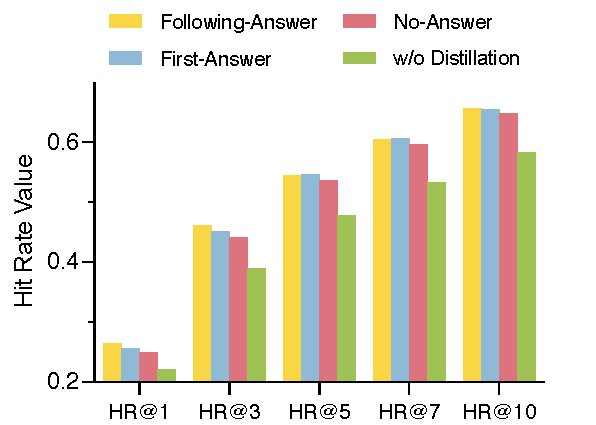
\includegraphics[width=0.45\textwidth]{latex/pic/fig4.pdf}
    \caption{The performance of retriever models across three types of training sets, which vary based on the initial appearance and placement of ground truth in the retrieved subsets.}
    \label{fig:04}
    \vspace{-10pt}
\end{figure}
Our previous experiment demonstrate that Rule-Based supervision signals, which places documents containing answers at the top, are ineffective and detrimentally impacting the retriever's performance.
This indicates that simply re-ranking documents based solely on the presence of ground truth (i.e., the correct answer) does not provide the high-quality text similarity insights required for effective distillation.
To delve deeper into the influence of the appearance and placement of ground truth in the re-ranking process, we categorize the initial retrieved document subsets $D_n$ based on \textit{NQ}'s queries into three categories:
(1) \textit{Following-Answer}: contains at least one document with the correct answer, but this kind of document is not at the first position in the subset. 
This data type is used in our experiments detailed in Section \ref{sec:4}.
(2) \textit{First-Answer}: contains at least one document with the correct answer, and this kind of documents is at the first position in the subset.
(3) \textit{No-Answer}: no documents in the subset contain the correct answer.

We follow the same training setting used in our primary experiments in Section \ref{sec:4}, and use GPT-4 Turbo as the LLM teacher model.
% The performance of the retriever models under these three data types of training are shown in Figure \ref{fig:04}.
% The results indicate that subsets with having ground-truth documents (i.e., Following-GT and First-GT) significantly improve retriever performance more than those without (i.e., No-GT).
% distilling the retriever model using subsets of relevant documents that contain the ground truth (i.e., Follow-GT and First-GT) produces better results compared to using the types that do not contain the answer (i.e., No-GT), and using Follow-GT proves to be more effective than using First-GT overall. 
Together with findings from the \textit{Rule-Based} experiments in Section \ref{sec:4}, the experiment results shown in Figure \ref{fig:04} indicate that considering the semantic similarity of the text is far more important than arranging documents containing the answers to the top for re-ranking in distillation training, as even the retriever under the \textit{No-Answer} data set training has notable improvements.

Moreover, as the \textit{Following-Answer} training data, where the correct answers are not ranked first initially, yields better training results than using the the \textit{First-Answer} training data, indicating that optimizing the ground truth placement in re-ranking also has a positive effect on the experimental results after the consideration of text similarity.
% Combined with the results from the Rule-Based experiments, this experimental results show that both prioritizing documents containing the answers and considering the semantic similarity of the text beyond just the answers determine the quality of the re-ranking distillation signals.

% This results suggests that re-ranking information containing the ground truth, especially those not initially ranked first, is a more effective distillation method. 
% Moreover, even the retriever under the No-GT data set training has notable improvements, showing that which highlights the advanced ranking capabilities of LLMs.
% \vspace{-1mm}
\subsection{Impact of the Training Set Size} 
\label{sec:5-3}
Our previous experiments demonstrate that our distillation framework significantly enhances retriever model performance with just 1,000 training instances. 
In this subsection, we explore how different training set sizes affect distillation effectiveness.
We use training sets of of 50, 100, 200, 500, 1000, and 2000 data instances from the \textit{Following-Answer} data type, with other settings consistent with our experiments in Section \ref{sec:4}. 
In addition, we use GPT-4 Turbo as our LLM teacher model.
% In addition to this, we use the same training setting as Section \ref{sec:5-1} uses to train the retriever model, and the experimental results are shown in Figure \ref{fig:05}.

Results in Figure \ref{fig:05} show that the performance of the retriever model improves significantly with training data with thousands of or even only hundreds of instances.
These empirical findings highlight the data efficiency of our proposed distillation scheme.
% initial increases in performance are significant with small training sets. 
In addition, although initial performance increases are notable with small training sets, the rate of improvement decreases as more training data is used.
This pattern indicates a \textit{scaling law} in distillation training, where further enhancements become increasingly difficult as the model's performance improves.
For models that already perform well, even marginal improvements require much more data, demanding greater training resources.
\begin{figure}
    \centering
    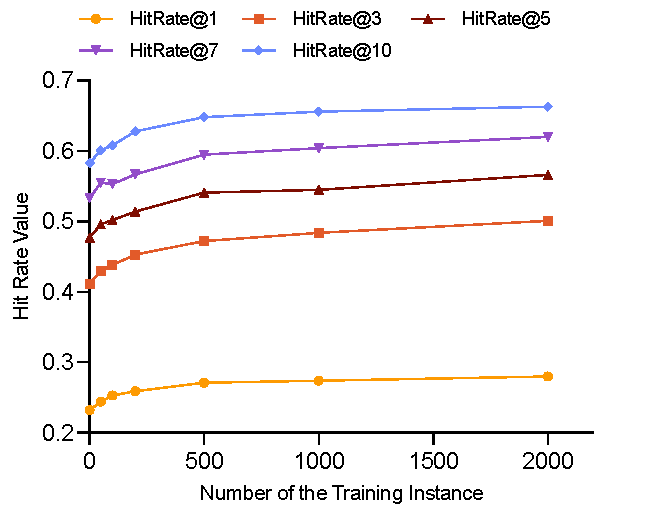
\includegraphics[width=0.5\textwidth]{latex/pic/fig5.pdf}
    \caption{The performance of retriever models under different training set size.}
    \label{fig:05}
    \vspace{-4mm}
\end{figure}

% For already high-performing retriever models, even small improvements require an exponentially larger amount of training data.
\subsection{Impact of the Re-ranking List Size}
\label{sec:5-4}
\begin{figure}[!htbp]
    \centering
    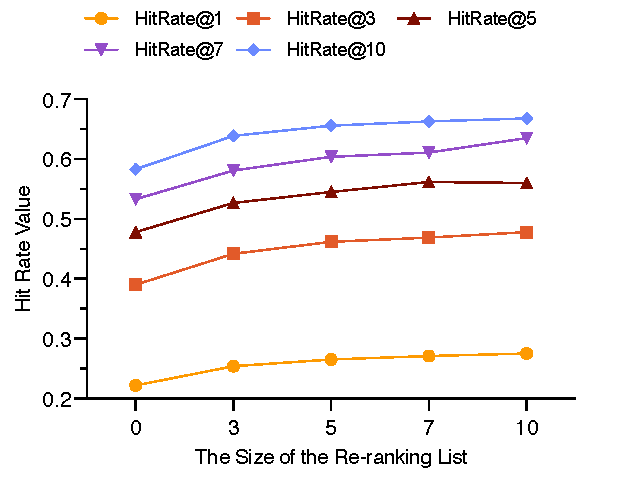
\includegraphics[width=0.5\textwidth]{latex/pic/fig6.pdf}
    \caption{The performance of retriever models under different size of the re-ranking list. The performance corresponding to 0 re-ranking list size represents the baseline retriever model performance.}
    \label{fig:06}
    \vspace{-4mm}
\end{figure}
In previous experiments, we set the re-ranking list to five documents (i.e., we retrieve five relevant documents each time).
Generally, larger re-ranking lists offer more supervision signals from LLMs, thus potentially enhancing the effectiveness of distillation training. 
To explore the impact of re-ranking list size on our distillation method, we vary the re-ranking list sizes, using the top-3, top-5, top-7, and top-10 documents from each relevant retrieved subset to conduct the distillation training.
% That is, during the initial data collection phase, the off-the-shelf retriever model returns the top-3, top-5, top-7, and top-10 relevant documents, respectively.
We keep other training settings consistent with those in our primary experiments in Section \ref{sec:4} and use GPT-4 Turbo as the LLM teacher model.

The experimental results shown in Figure \ref{fig:06} show that increasing the re-ranking list size progressively improves the effectiveness of the distillation training. 
As the list expands from re-ranking three documents to ten documents, the performance of the distilled retriever model consistently improves.
Moreover, compared with the retriever model's baseline performance, setting the size of the re-ranking list to 3 still significantly improves the retriever model's performance not only in HitRate@3 but also across broader metrics from HitRate@5 to HitRate@10.



% TODO in appendix:
% direct distill prompt cases
% case studies in metric v.s. LLM RAG performance
